\documentclass[12pt,letterpaper]{article}

%%%%% CAMBIAR LA PRIMERA LINEA POR LA SIGUIENTE PARA LA MEMORIA DE PROYECTO %%%%%
%\documentclass[12pt,letterpaper,oneside]{book}

% Paquetes basicos ...
\usepackage[utf8]{inputenc} % OJO!!!  => MANTENER ESTA LINEA PARA FACIL CONVERSION A WORD EN EL FUTURO ...
\usepackage[spanish]{babel}
\usepackage{graphicx} 
\usepackage{array}
\usepackage{tabularx}
\usepackage{amssymb, amsmath}

% Paquetes extras ... 
\usepackage{subfigure}
\usepackage{color}
\usepackage{anysize} 
\usepackage{breakcites}
\usepackage{enumitem}

\usepackage{hyperref}

\begin{document}
\marginsize{2.5cm}{2cm}{2cm}{2cm} 

% Para que no aparezca la numeracion en el pie de pagina de todo el documento ...
%\pagestyle{empty}


%%%%%% ******  INICIO CARATULA ***** %%%%%%%%%
% Especificaciones de la caratula PPG
\begin{titlepage}
\begin{center}
\vspace*{-0.5in}
\begin{large}
\textbf{UNIVERSIDAD MAYOR DE SAN ANDRÉS}\\
\vspace*{0.15in}
\textbf{FACULTAD DE INGENIERÍA}\\
\vspace*{0.15in}
\textbf{CARRERA DE INGENIERÍA ELECTRÓNICA}\\
\vspace*{0.1in}
\end{large}
% Logo UMSA
\begin{figure}[htb]
\begin{center}

\includegraphics[width=8cm]{umsa.jpg}
\end{center}
\end{figure}
\begin{Large}
\textbf{PERFIL DE PROYECTO DE GRADO} 
\end{Large}
\vspace*{0.4in}

\begin{normalsize}
\textbf{``Aprendizaje fin a fin para la conducción autónoma de vehículos domésticos usando visión artificial y redes neuronales convolucionales''} \\
\end{normalsize}

\vspace*{0.2in}

\begin{large}
\textbf{POSTULANTE:} JOSE EDUARDO LARUTA ESPEJO\\
\end{large}

\begin{large}
\hspace{0.08in} \textbf{TUTOR:} JAVIER SANABRIA GARCIA\\
\end{large}

\begin{large}
\hspace{0.44in} \textbf{D.A.M.:} GONZALO SAMUEL CABA MORALES\\
\end{large}

\vspace*{0.2in}

\begin{normalsize}
LA PAZ, NOVIEMBRE 2018\\
\end{normalsize}
\end{center}
\end{titlepage}


\thispagestyle{empty}
% Generacion del indice
\tableofcontents
\newpage

%%%%%% ******  FIN CARATULA ***** %%%%%%%%%

% Contenido del PPG
% NOTA: presionar F11 para que se actualicen las citas bibliograficas ...

\section{Introducción}

Los vehículos autónomos han pasado de ser un tema de ciencia ficción a convertirse una realidad cada vez más 
cercana. Si bien existe un recorrido muy largo para llegar a implementar sistemas completamente autónomos en las calles, 
los recientes avances en la tecnología junto con el interés económico de grandes empresas y corporaciones en el mundo 
ha hecho posible incluir diversos niveles de autonomía a vehículos con fines de uso doméstico e industrial con éxito.

Una de las áreas que más se ha nutrido de los recientes avances es el área de la visión artificial o visión por computador; 
resolviendo con facilidad tareas de una complejidad muy alta, como la detección y reconocimiento de objetos. 
Este crecimiento, en gran parte, se ha debido al desarrollo y optimización de las redes neuronales, las cuales se han 
constituido en una herramienta con muchas potencialidades y aplicaciones por la forma en la que se procesa la información 
y su capacidad para generalizar tareas complejas en base a una gran cantidad de datos de entrenamiento. En específico, 
las redes neuronales convolucionales han podido revivir al campo de la visión artificial gracias a la forma eficiente 
en la se que procesan imágenes o matricies multidimensionales y la capacidad de crear representaciones internas a partir 
de filtros de convolución en las capas ocultas de la red neuronal\cite{krizhevsky2012imagenet}.

La visión artificial juega un papel muy importante en el desarrollo de vehículos autónomos por cuanto permite 
procesar imágenes digitales provenientes de cámaras instaladas en los mismos vehículos y extraer información 
valiosa para la navegación y la conducción, como ser la detección de carril, peatones, signos de tránsito, otros vehículos, 
etc. Esta utilidad hace posible diversas oportunidades de investigación y desarrollo de algoritmos y sistemas de visión 
artificial orientados a conducción autónoma.

El presente proyecto se centra en el desarrollo de un sistema de conducción autónoma basado en visión artificial para 
la generación de comandos de control para la conducción autónoma de un vehículo doméstico con un modelo de locomoción 
de Ackerman. Se intenta desarrollar un sistema de aprendizaje “fin a fin” que consta de un modelo de predicción 
que genera comandos de control a partir de un estímulo visual proveniente de una cámara monocular.
%% detallar un poco mas el reto del sistema fin a fin

% definicion de sistemas fin a fin

% TODO: referencias 
\section{Antecedentes}

El primer intento de desarrollo de un sistema de conducción autónomo “fin a fin” fue llevado a cabo por la Agencia 
de Proyectos de Investigación Avanzada en Defensa de los Estados Unidos (DARPA) con un proyecto conocido 
como el Vehículo Autónomo de DARPA o DAVE \cite{lecun2004dave} en el cual un vehículo radio controlado a escala tenía la 
tarea de conducir a través de un entorno escabroso. El vehículo DAVE fue entrenado a partir de cientos de
horas de conducción humana en entornos similares pero no idénticos. Los datos de entrenamiento 
incluyeron imágenes de dos cámaras de video y comandos de control generados por un operador humano. 

Paralelamente a este esfuerzo realizado por el DARPA y debido a la limitada capacidad computacional de la época, 
los avances en las distintas tareas que componen la conducción autónoma se han enfocado en el tratamiento de las señales 
y datos provenientes de los sensores con algoritmos de procesamiento básicos llegando a crearse implementaciones efectivas 
basadas en un flujo de trabajo descrito a continuación.

\subsection{Sistemas de Conducción Autónoma}
Un sistema de conducción autónoma es una combinación de varios componentes o subsistemas donde las tareas 
de percepción, toma de decisiones y operación de un vehículo son desarrolladas por un sistema electrónico en lugar
de un conductor humano. 

El primer hito en el desarrollo de un sistema completamente autónomo vino 
con la organización del DARPA “Grand Challenge” en el cual equipos de varias universidades, 
institutos de investigación y empresas tuvieron que enfrentar el difícil reto de desarrollar 
un sistema capaz de controlar un vehículo doméstico a través de una carretera 
ripiada en medio del desierto de Arizona. Dentro las 2 versiones del Darpa Grand Challenge 
destacaron los proyectos de universidades como Stanford con el robot Stanley \cite{Thrun2006} que fue el primer 
vehículo en recorrer mas de 170 kilómetros en una carretera ripiada de manera completamente autónoma. 

% IMAGEN: stanley de stanford

%%%% Figura 1 %%%%%%
\begin{figure}[!h] 
\centering
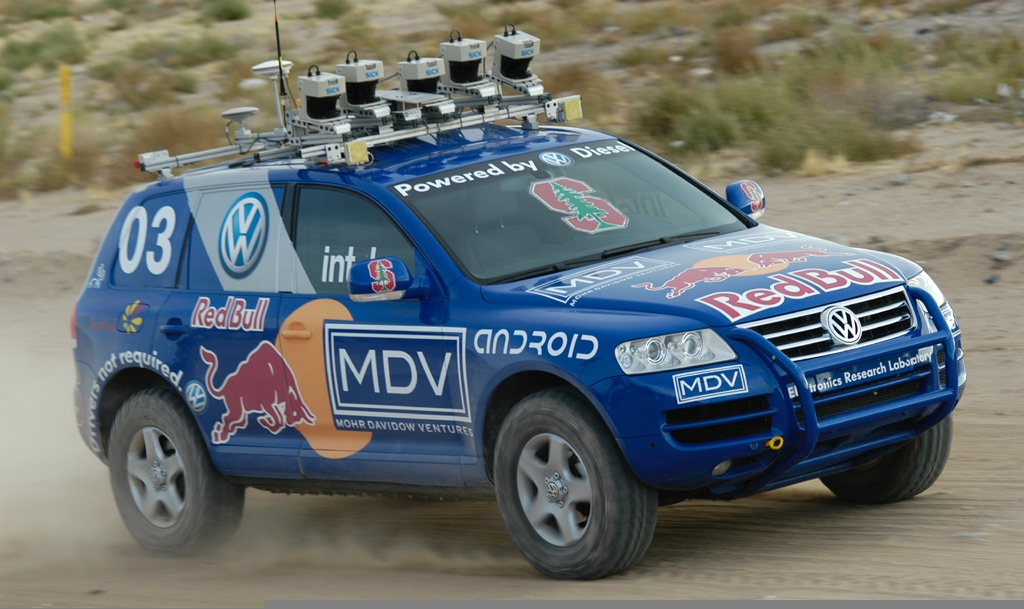
\includegraphics[width=0.5\textwidth]{stanley1}
\caption{Stanley, el vehículo autónomo de Stanford que ganó la competencia DARPA Grand Challenge en 2005. 
        Fuente: \href{http://stanford.edu/~cpiech/cs221/apps/driverlessCar.html}{stanford.edu} }
\label{fig:stanley1}
\end{figure}

El éxito de los proyectos que participaron en el grand challenge sentó un gran precedente en el desarrollo de lo que 
ahora se conoce como \textit{Self Driving Car} o vehículo autónomo. De hecho, muchos de los equipos 
participantes de este concurso se constituyen en la actualidad como existosas empresas de desarrollo o 
coadyuvan en iniciativas privadas de gigantes de la tecnología como Google, Uber o Nissan.

Sin embargo, debido al creciente interés tanto en investigación como económico en los sistemas de conducción 
autónoma, la Sociedad de Ingenieros en Automoción (SAE por sus siglas en inglés) ha elaborado un estándar donde se 
detallan distintos aspectos concernientes. La regulación define varios niveles de autonomía en 
vehículos terrestres, aéreos y acuáticos yendo desde un control completamente manual, 
normalmente observado en vehículos completamente mecánicos, pasando por asistencias al control 
hasta llegar a un vehículo completamente autónomo en todas sus tareas

% IMAGEN: niveles de autonomia
%%%% Figura 2 %%%%%%
\begin{figure}[!h] 
\centering
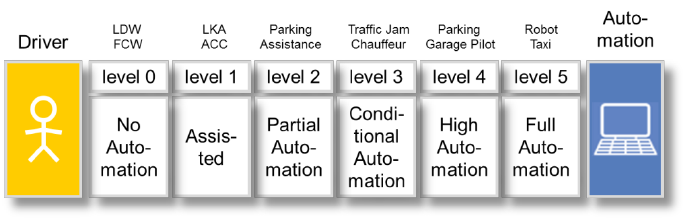
\includegraphics[width=0.70\textwidth]{levels}
\caption{Niveles de automatización en la conducción según SAE. 
        Fuente: \href{https://www.researchgate.net/figure/Terms-related-to-automated-driving-according-to-SAE-and-VDA_fig1_273883061}{researchgate} }
\label{fig:levels}
\end{figure}

La creación de estándares y regulación ha tenido como consecuencia que, en la actualidad, existan varias iniciativas 
en el desarrollo de los \textit{self Driving Cars}, siendo una de las más 
importantes la empresa Waymo, dependiente de Google a través de su empresa Pública Alphabet. Waymo, ha aprovechado 
el uso de tecnologías emergentes de sensado como el LIDAR para mejorar el mapeo y la navegación a través de algoritmos 
de fusión de sensores. Aparte de Alphabet, existen diversas iniciativas privadas en el desarrollo de vehículos autónomos 
con fines comerciales como los Self Driving Cars de Uber, Toyota, BMW, Ford, entre otros.

% IMAGEN: vehiculo de waymo

%%%% Figura 1 %%%%%%
\begin{figure}[!h] 
\centering
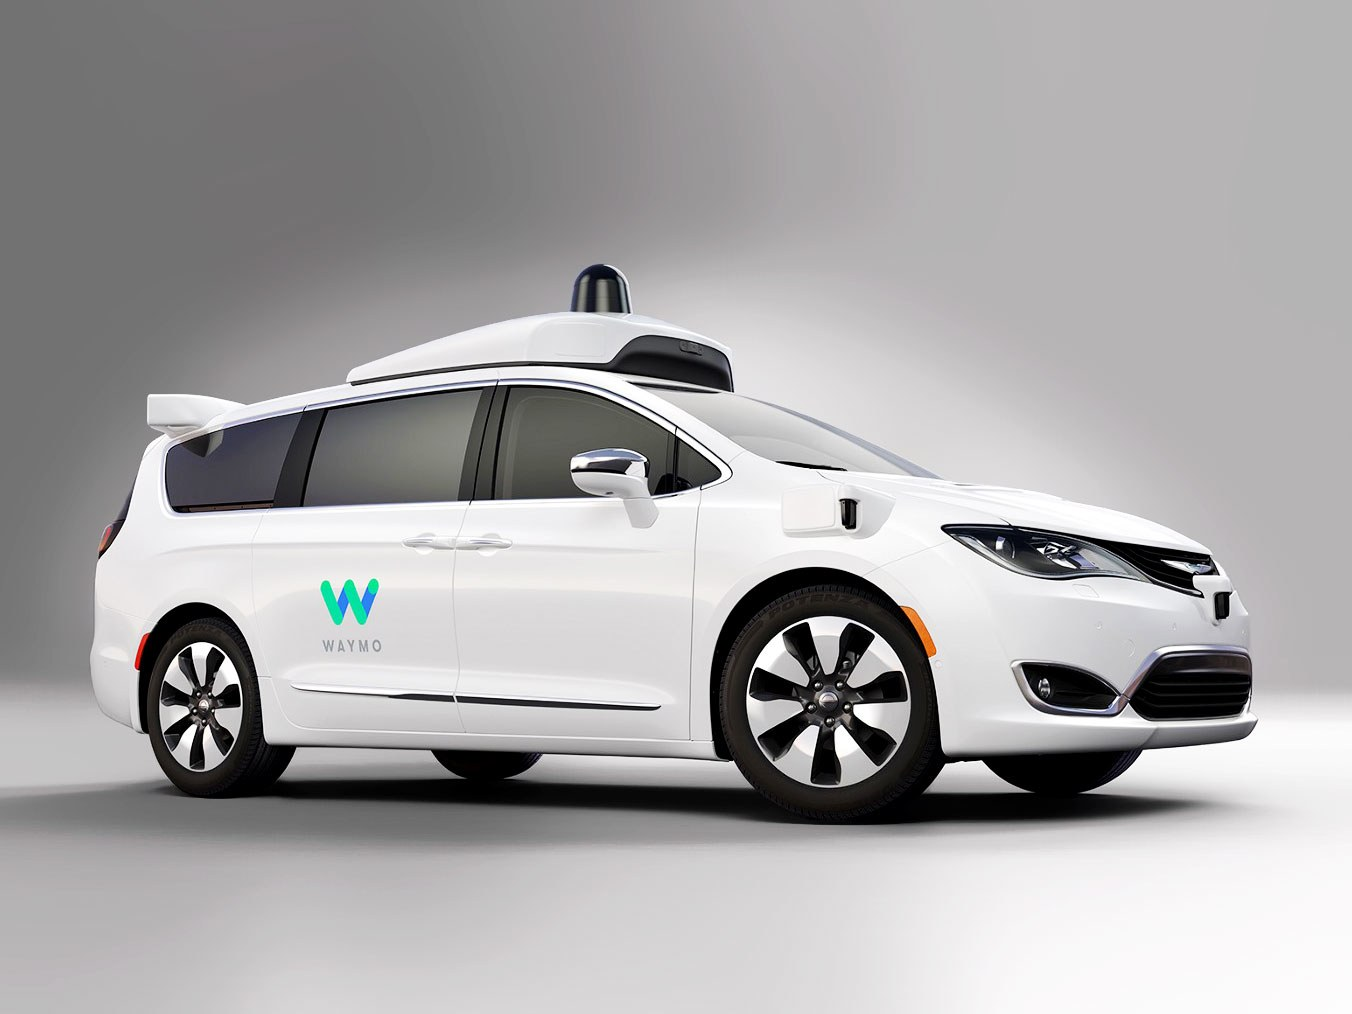
\includegraphics[width=0.5\textwidth]{waymo}
\caption{El vehículo autónomo de Waymo. 
        \href{https://waymo.com/}{waymo.com}}
\label{fig:waymo}
\end{figure}

Una de las tareas más importantes dentro de un \textit{self driving car} es la detección y mantención del carril del 
vehículo. Fabricantes de vehículos automotores han incluido con éxito sistemas de asistencia al conductor para la 
mantención del carril usando cámaras digitales y visión artificial para poder detectar la posición del automóvil con 
respecto al carril. Estos sistemas se consideran fundamentales en sistemas de conducción autónoma. Durante las últimas 
dos décadas, se han desarrollado distintos tipos de sistemas y enfoques para resolver el problema de la mantención de 
carril.

\subsubsection{Arquitectura general de un sistema de conducción autónoma}
En general, la arquitectura de un sistema de conducción autónoma se puede entender como la integración de varios módulos o 
subsistemas funcionales que operan en coordinación tal como se puede observar en la Figura(\ref{fig:esquema}). 

% IMAGEN: arquitectura

%%%% Figura 1 %%%%%%
\begin{figure}[!h] 
    \centering
    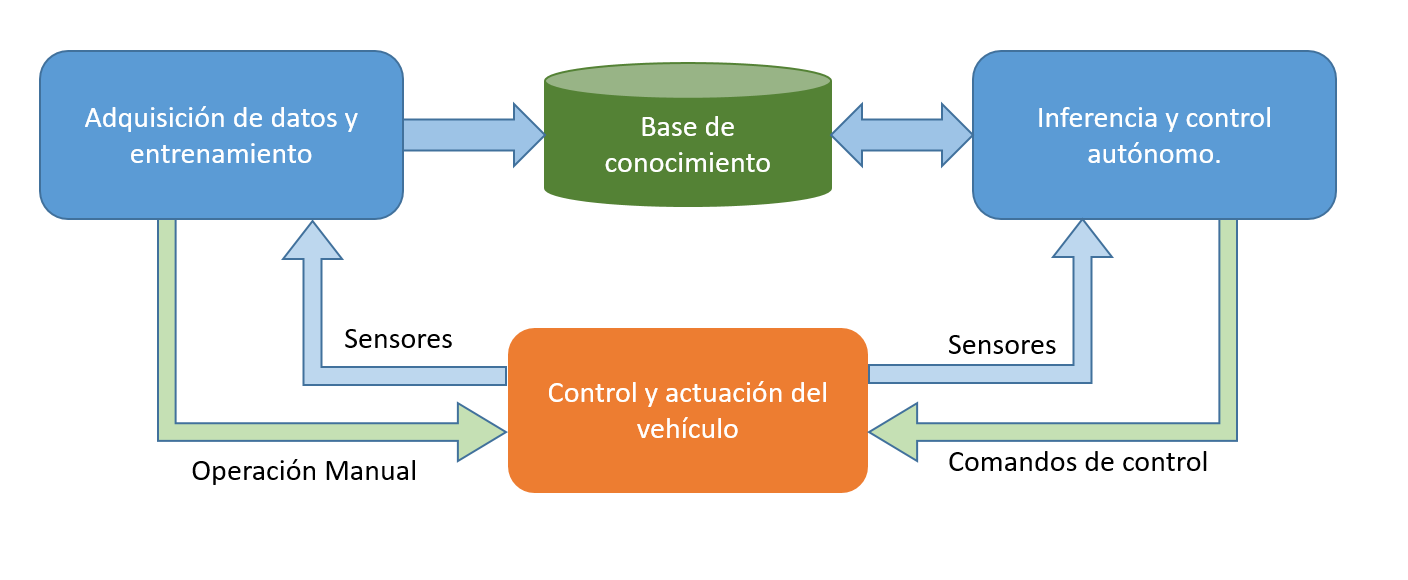
\includegraphics[width=0.75\textwidth]{img/esquema}
    \caption{Arquitectura de un sistema de conducción autónoma. Fuente: Elaboración propia.}
    \label{fig:esquema}
    \end{figure}


Normalmente, este tipo de sistemas cuenta con una etapa de adquisición de datos y entrenamiento que servirá para 
alimentar una base de conocimiento o reglas en las que se basará el módulo de inferencia y control autónomo. 
Asimismo, tanto el subsistema de adquisición de datos y entrenamiento como el subsistema de inferencia y 
control autónomo interactuan directamente con el subsistema de control y actuación del vehículo. 

Los mayores esfuerzos se han enfocado principalmente al desarrollo del subsistema de inferencia y 
control autónomo ya que es el que define el rendimiento de un sistema de conducción autónoma en sí. 
Este subsistema, a su vez, puede ser analizado como un conjunto de varios módulos que interactúan 
entre sí de manera secuencial, como se puede apreciar en la Figura(\ref{fig:inferencia}). 



\subsubsection{Sistemas de aprendizaje fin a fin}
Tradicionalmente, los sistemas de aprendizaje requieren de múltiples etapas de procesamiento que interactuan entre sí, como se 
muestra en la Figura(\ref{fig:inferencia}). Por su parte, los sistemas de aprendizaje fin a fin intentan condensar 
estas etapas de procesamiento y reemplazarlas usualmente con una sola red neuronal. Estos sistemas han demostrado ser 
altamente efectivos en contraste a los enfoques tradicionales, principalmente porque abstrae y resumen el diseño de las 
etapas intermedias de un sistema de aprendizaje tradicional con una sola etapa. La desventaja de los 
sistemas de aprendizaje fin a fin radica en la necesidad de grandes cantidades de datos de entrenamiento 
en comparación con los enfoques tradicionales, sin embargo, gracias a la gran disponibilidad de datos de entrenamiento y 
la accesibilidad de instrumentos y herramientas de adquisición de datos, esta desventaja no representa una dificultad de 
gran magnitud en el desarrollo de sistemas fin a fin. 

Los sistemas de aprendizaje fin a fin se han explorado de manera exitosa en los últimos años, esto debido a la creciente
disponibilidad de sistemas de cómputo de alta concurrencia, en especial las Unidades de Procesamiento Gŕafico de propósito
general o GPGPU por sus siglas en inglés. Esta disponibilidad ha logrado que se puedan entrenar redes neuronales completas 
en una estación de trabajo que no consume demasiada energía. Una de las empresas pioneras en GPGPU es Nvidia con su herramienta 
CUDA, que ha permitido el desarrollo de algoritmos de entrenamiento e inferencia para redes neuronales de manera sencilla. Es 
precisamente Nvidia que ha demostrado que los sistemas de aprendizaje fin a fin pueden tener éxito con el desarrollo de un 
prototipo y arquitectura de vehículo autónomo \cite{bojarski2016end}.


%*******************JUSTIFICACION*******************

\section{Justificación del Proyecto}

\subsection{Justificación académica}

Desde el punto de vista académico, el proyecto se justifica en el entendido del uso de técnicas y procedimientos 
de ingeniería para el análisis y diseño de un sistema de aprendizaje “fin a fin” usando redes neuronales y una plataforma 
para el entrenamiento y despliegue del mismo. Tales técnicas y procedimientos incluyen la definición de 
la arquitectura de la red neuronal, el entrenamiento y el análisis del rendimiento de la misma. Así como 
también el dimensionamiento de los componentes de cómputo embebido para el prototipo y la implementación de 
los sistemas de control electrónico de bajo nivel para el mismo. Tales técnicas y 
procedimientos se corresponden de manera integral con los conocimientos adquiridos a lo largo de la carrera 
de Ingeniería Electrónica en sus distintas asignaturas.

\subsection{Justificación tecnológica}

Dada la creciente relevancia de los sistemas autónomos en la actualidad, el proyecto se justifica 
desde el punto de vista tecnológico dado que se presenta la aplicación de nuevas
herramientas y plataformas de software para el desarrollo de sistemas de autónomos, visión por computador 
y redes neuronales convolucionales, que representan áreas vigentes en la investigación tecnológica hoy en día.

El sistema desarrollado se constituirá a su vez en una plataforma de desarrollo sobre el cual se podrá 
extender su funcionalidad y mejorar sus resultados usando herramientas de software de fácil acceso y aprendizaje 
presentando la posibilidad de continuar y extender la investigación en sistemas de conducción autónoma, robótica móvil, 
visión por computador y aprendizaje profundo.

\subsection{Justificación técnica}

Desde el punto de vista de las técnicas aplicadas, el proyecto se justifica dado que se pretende presentar una técnica 
alternativa al enfoque tradicional en el desarrollo de sistemas de aprendizaje, presentando el desarrollo de un sistema 
de aprendizaje fin a fin, que facilitará su análisis, diseño, entrenamiento y puesta en marcha en futuros proyectos 
de investigación y aplicaciones en distintas áreas de la ingeniería. 

La propuesta de la nueva técnica de aprendizaje fin a fin representa un avance en relación al desarrollo de sistemas 
tradicionales por su impacto en el requerimiento de recursos y de conocimiento específico requerido.


%******************ANALISIS DE LA PROBLEMATICA*********************
%------ TODO: completar esta parte ------------- %
\section{Análisis de la problemática y \\
planteamiento del problema}
\subsection{Análisis de la problemática}
% PROBLEMATICA: Conjunto de aspectos que causan problemas en un PG.
% ANALISIS DE LA PROBLEMATICA: Determinacion de las causas sus efectos y sus relaciones, vinculados con los aspectos problematicos de la idea del proyecto.  
% ****Es el analisis de las cuestiones discutibles que requieren de una solucion en el PG.

Se han estudiado diferentes enfoques para lograr solucionar la tarea de 
conducción autónoma para vehículos domésticos usando sistemas de aprendizaje. Normalmente, la salida del 
sistema se expresa como una serie de comandos de control de aceleración y dirección 
del volante del vehículo. Estos comandos se pueden obtener de diversas maneras dependiendo 
el nivel de robustez y abstracción que el sistema requiere. Muchos sistemas 
se basan en la fusión de distintos tipos de sensores y fuentes de información como ser 
mapas satelitales, GPS, sensores láser y cámaras. La combinación de esta información 
es procesada y fusionada mediante distintos algoritmos de filtrado tales como el filtro de kalman. 
La característica de este tipo de sistema es que se puede expresar como una serie de etapas 
de procesamiento mediante el cual la información fluye y se transforma, cada una de las etapas es 
diseñada e implementada en base a conocimiento específico y con requerimientos y limitaciones específicas 
de la tarea que realiza tal como se puede apreciar en la Figura(\ref{fig:inferencia}).

Si bien el enfoque anteriormente mencionado ha logrado conseguir importantes avances y resultados 
muy prometedores, involucra un gran esfuerzo a la hora de diseñar cada una de las etapas independientemente 
para luego hacer que funcionen todas juntas y cumplan la tarea asignada. Este proceso usualmente requiere 
de un equipo de expertos que sea capaz de realizar las tareas de diseño de las etapas o módulos del sistema 
y el de la integración de los módulos en un solo sistema funcional. Este enfoque, pese a que ha demostrado ser 
una forma efectiva de trabajo para diversos problemas, tiene la desventaja de requerir muchos 
recursos y tiempo para poder lograr un sistema funcional. 

%
\subsection{Planteamiento del problema}
% PLANTEAMIENTO DEL PROBLEMA: Tiene que ver con enfocar la solucion de los aspectos problematicos tratados, 
% desde su situacion inicial hasta su situacion final deseada.

% definir el concepto de informacion con referencia a datos
% 
De acuerdo a lo establecido anteriormente, se puede considerar a la etapa de inferencia y control autónomo de 
un sistema de conducción autónoma como un sistema de procesamiento de información que consta de varias etapas 
secuenciales que transforman la información de acuerdo a parámetros previamente establecidos. Se debe tener en 
cuenta varios aspectos concernientes tanto al diseño como a la implementación de dichos tipos de sistemas. 

%%%% Figura 1 %%%%%%
\begin{figure}[!h] 
    \centering
    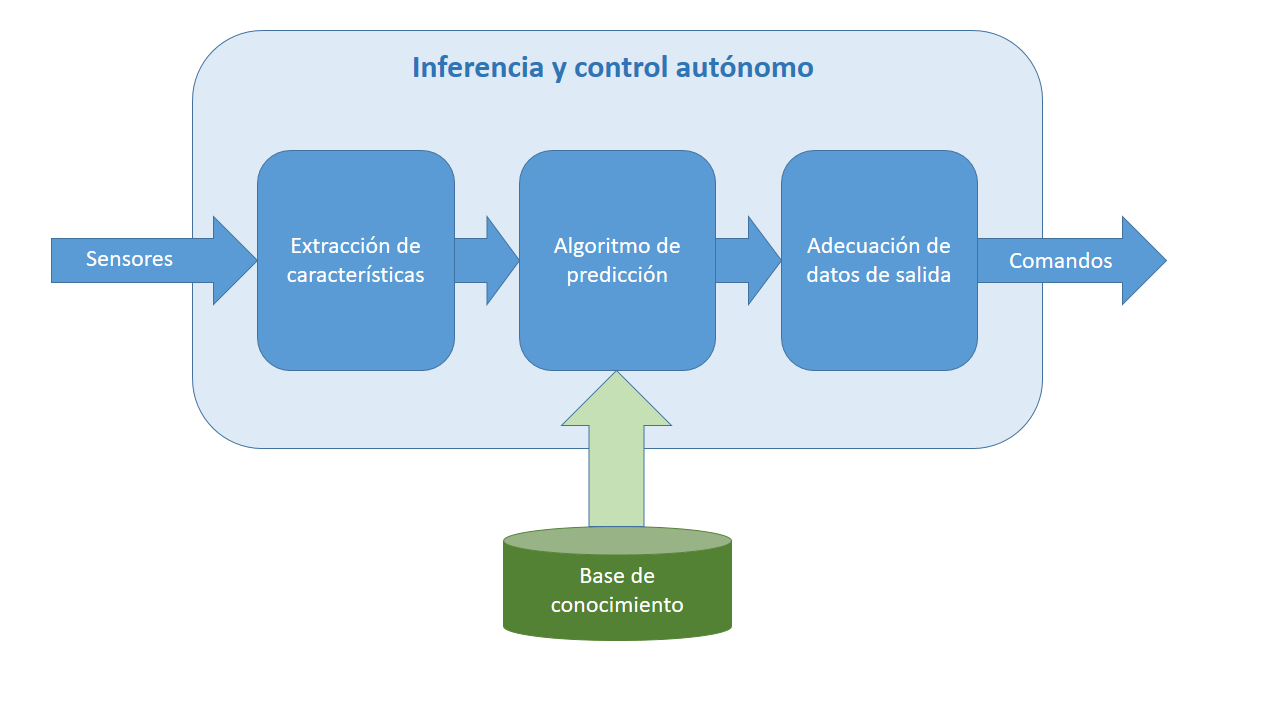
\includegraphics[width=0.75\textwidth]{img/inferencia}
    \caption{Componentes del subsistema de inferencia y control autónomo. Fuente: Elaboración propia.}
    \label{fig:inferencia}
\end{figure}


En el área de visión por computadora para tareas de conducción autónoma, normalmente se sigue el siguiente 
flujo en el desarrollo un sistema o prototipo:

\begin{enumerate}
    \item \textbf{Extracción de características.} Esta etapa incluye el preprocesamiento y transformación de la imagen 
    en un conjunto de características de distinta índole. Estas características se suelen llamar también descriptores 
    y sirven para describir los aspectos más relevantes de la imagen para la tarea final, por ejemplo, la detección de bordes. 
    La extracción de características también se usa para reducir la dimensionalidad inicial de la imagen a una más tratable y 
    amigable con la capacidad de procesamiento computacional disponible. Las características o descriptores a usarse 
    se definen manualmente por medio de conocimiento experto y se afinan de la misma manera.

    \item \textbf{Algoritmo de predicción.} Esta etapa incluye típicamente un algoritmo de aprendizaje previamente 
    entrenado con un conjunto de datos adecuado, permite realizar distintas tareas de alto nivel sobre los descriptores 
    obtenidos de la imagen. Estas descripciones de alto nivel incluyen normalmente tareas de detección, 
    clasificación o regresión. Los algoritmos de aprendizaje incluyen típicamente algoritmos básicos, tales como árboles de decisión,
    regresión lineal o máquinas de soporte vectorial ya que deben realizar la tarea de predicción en un 
    conjunto de dimensionalidad relativamente baja (los descriptores).

    \item \textbf{Adecuación de los datos de salida.} La información extraída de la anterior etapa debe 
    procesarse para poder ser traducida a comandos de control que actuen directamente con las etapas 
    de bajo nivel del vehículo, es decir la etapa de actuación y potencia. En esta etapa se suele incluir algún algoritmo 
    de control realimentado para el control de motores así como también algoritmos de fusión de distintas fuentes de información
    para obtener finalmente una señal de comando para los actuadores.
\end{enumerate}

Como se ha podido observar, el flujo de trabajo en un sistema de conducción autónomo se compone de varias etapas 
secuenciales que se deben realizar con conocimiento y experiencia específica en cada una de las mismas. 

Por su parte, otra de las dificultades con este acercamiento, al reto de la conducción autónoma es el de la reducida
flexibilidad del sistema. En otras palabras, si se quisiera modificar el sistema para agregar requerimientos o 
expandir la funcionalidad del mismo, se debe realizar una modificación a la etapa específica y evaluar el impacto de 
las modificaciones en todo el sistema en su conjunto. Esto dificulta de manera sustancial la reutilización de diversos
componentes en sistemas similares.

Finalmente, la exagerada complejidad y conocimientos requeridos para poder implementar un sistema experimental 
de esta naturaleza hace prácticamente imposible su desarrollo por equipos de investigación pequeños o investigadores 
individuales. Dada la importancia y la potencialidad de los sistemas de conducción autónoma es escencial reducir 
esta dificultad de implementación y experimentación.

En conclusión, el desarrollo de un sistema de conducción autónoma presenta tres principales dificultades a la hora de 
ser abordado: 
\begin{enumerate}
    \item Conocimiento experto de cada una de las etapas involucradas en el sistema.
    \item Poca flexibilidad en el diseño y la implementación del sistema una vez establecido y probado.
    \item El tiempo y recursos necesarios para poder diseñar e implementar un sistema de tal naturaleza lo hace privativo para equipos de investigación pequeños o con poco presupuesto.
\end{enumerate}
%------------------
\section{Objetivos}
\subsection{Objetivo General}

Diseñar un sistema de aprendizaje “fin a fin” capaz de generar de comandos de 
control de vehículos domésticos basado en visión artificial y redes neuronales 
convolucionales para facilitar el diseño e implementación de sistemas de conducción autónoma.

\subsection{Objetivos Específicos}
Para alcanzar el objetivo general será necesario:


\begin{itemize}

    \item Estudiar los aspectos concernientes al desarrollo de sistemas de conducción autónoma y sistemas de aprendizaje.
    \item Analizar los requerimientos de un sistema de conducción autónoma capaz identificar y mantener su carril mientras se conduce.
    \item Diseñar la arquitectura de un sistema de conducción autónoma en base a los requerimientos previamente establecidos.
    \item Diseñar el subsistema de adquisición de datos y entrenamiento para tareas de conducción autónoma.
    \item Diseñar el subsistema de control y actuación para la conducción autónoma de un vehículo con características similares a las de un vehículo doméstico real.
    \item Diseñar el subsistema de inferencia y control autónomo basado en el uso de redes neuronales convolucionales.
    \item Analizar los resultados del entrenamiento e implementación del subsistema de inferencia y control autónomo.
    \item Realizar pruebas de rendimiento y análisis comparativos en el sistema implementado.

\end{itemize}


\section{Alcance}

El presente proyecto de grado cubre los siguientes aspectos dentro de su alcance:

\begin{itemize}
    \item El enfoque del estudio de sistemas de conducción autónomos de vehículos terrestres con el modelo de Ackermann.
    \item Investigación de arquitecturas y plataformas de software para el
    diseño y despliegue de robots móviles y tareas de conducción autónoma.
    \item El desarrollo del sistema se contempla en el marco de un proyecto académico 
    y, por tanto, será implementado usando herramientas de software comúnmente utilizadas en 
    investigación de sistemas autónomos.
\end{itemize}

El alcance detallado previamente estará acotado a su vez por una serie de supuestos.

\section{Límites}
El sistema, por su parte, contará con ciertas restricciones detalladas a 
continuación:
\begin{itemize}
    \item La tarea de conducción autónoma estará enfocada exclusivamente al 
    seguimiento y mantención del carril basado en imágenes provenientes de una cámara 
    sin considerar el reconocimiento e interpretación de otro tipo de información como 
    señales de tránsito, cruces e intersecciones o la presencia de peatones, ciclistas, 
    animales y otros objetos en la ruta.
    \item El prototipo a escala servirá solamente para un análisis superficial 
    de la dinámica de un vehículo automotor doméstico tomando como punto 
    de inicio modelos matemáticos simplificados y limitaciones de rangos de trabajo dentro 
    de dichos modelos.
    \item El diseño de la arquitectura de la red neuronal estará orientado a 
    tareas de aprendizaje supervisado y aproximación de funciones y limitado por la capacidad de 
    procesamiento disponible en el momento de la realización del presente proyecto.
\end{itemize}

\section{Solución Propuesta}

La propuesta del presente proyecto consta del desarrollo de un sistema de aprendizaje
fin a fin para la conducción autónoma de vehículos automotores domésticos. En este
sentido, se puede desglosar la arquitectura del sistema propuesto dividido en 
distintos subsistemas funcionales.

Por su parte, también es importante mencionar que el sistema en su conjunto contará 
con tres subsistemas que podrán interactuar entre sí: Subsistema de adquisición de datos y 
entrenamiento, subsistema de inferencia y conducción autónoma, subsistema de control 
y actuación como se puede apreciar en la Figura(\ref{fig:nuevo_esquema}).

\begin{figure}[!h] 
    \centering
    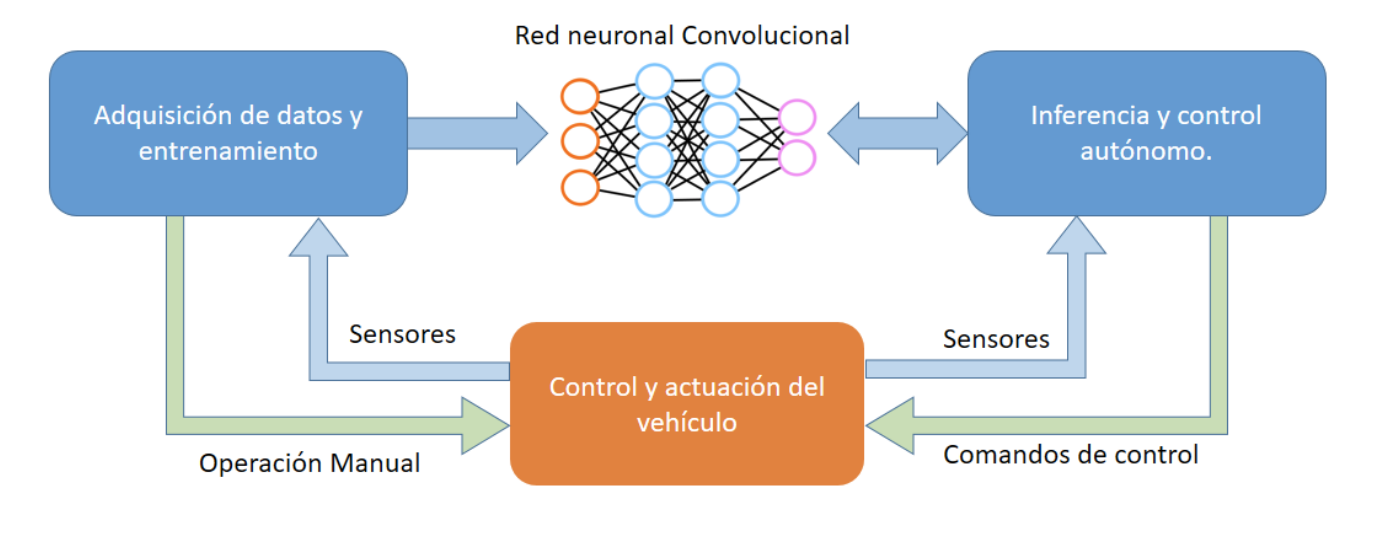
\includegraphics[width=0.80\textwidth]{img/nuevo_esquema}
    \caption{Arquitectura del sistema de conducción autónoma propuesto. Fuente: Elaboración propia.}
    \label{fig:nuevo_esquema}
\end{figure}

\subsection{Subsistema de adquisición de datos y entrenamiento.}
Este subsistema se compone de un conjunto de herramientas y utilidades para la 
adquisición de un nuevo conjunto de datos de entrenamiento y validación, así como
también un módulo de entrenamiento de la red neuronal convolucional para la tarea de
la generación de comandos de control.

\subsection{Subsistema de inferencia y conducción autónoma.}
El subsistema de inferencia y conducción autónoma tiene la tarea de obtener y ejecutar
las predicciones de la red neuronal entrenada en el Sistema de Adquisición de Datos y Entrenamiento.
Este subsistema tomará como entradas los datos de imágenes de una cámara y datos de 
sensores a bordo del prototipo para generar comandos de control acordes con el entorno
percibido. Este subsistema estará implementado en forma de un programa de ``piloto automático''
capaz de conducir el prototipo de manera autónoma.

\begin{figure}[!h] 
    \centering
    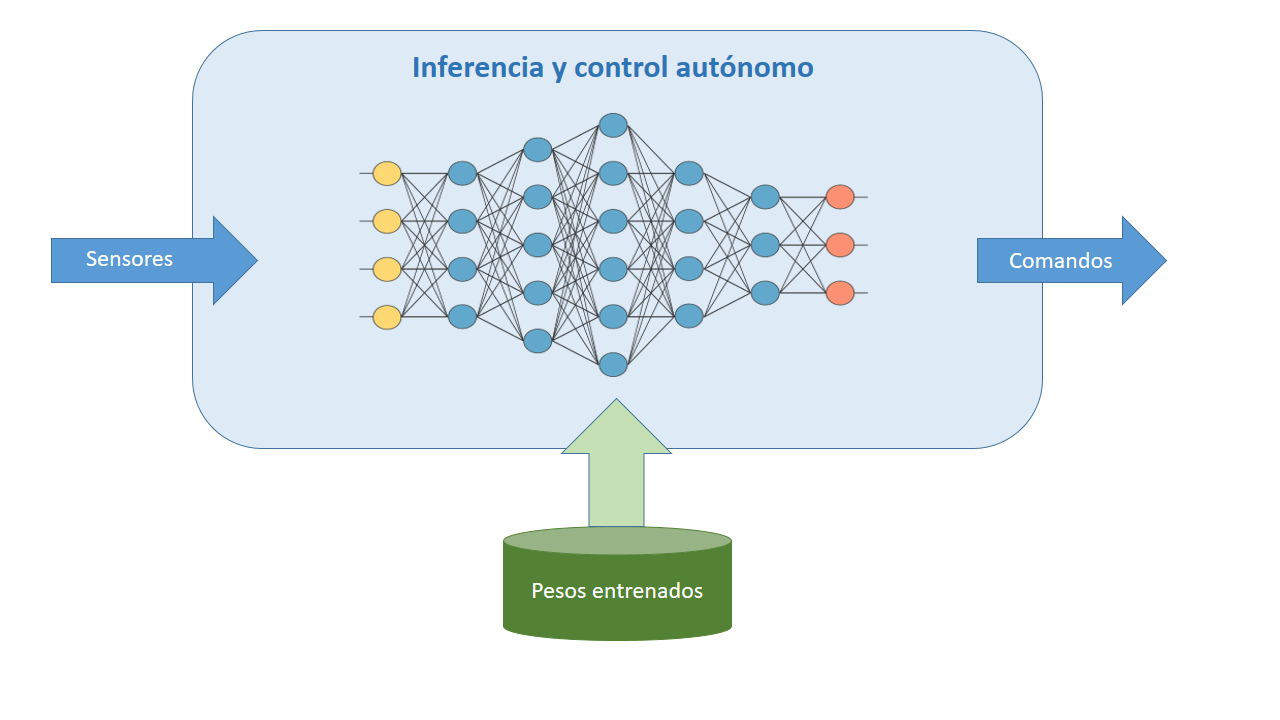
\includegraphics[width=0.75\textwidth]{img/nueva_inferencia}
    \caption{Subsistema de inferencia y control autónomo propuesto usando una red neuronal convolucional. Fuente: Elaboración propia.}
    \label{fig:nueva_inferencia}
\end{figure}


\subsection{Subsistema de control y actuación.}
Este subsistema compone la parte física de la propuesta. Contará con un modelo físico
a escala con locomoción de Ackermann con actuadores para la tracción y la dirección. 
Además, también contará con una plataforma electrónica embebida que se conectará 
directamente a los actuadores a través de una etapa de potencia y a los sensores 
correspondientes mediante un sistema de tiempo real. La parte lógica estará implementada
en una computadora de abordo que servirá de puente entre el mundo físico y la parte 
lógica de todo el sistema.

\section{Temario del Proyecto}
A continuación se presenta el temario tentativo de la memoria del proyecto, 
considerando los posibles contenidos, sin un detalle exhaustivo de los mismos 
puesto que podría ser una limitante en la estructura final. 
Inicialmente se considera la siguiente estructura:\\

\begin{itemize}

\item \textbf{Título.}

\item \textbf{Resumen.}

\item \textbf{Dedicatoria.}

\item \textbf{Agradecimientos.}

\item \textbf{Lista de Figuras.}

\item \textbf{Capitulo 1: Introducción}  

\item \textbf{Capitulo 2: Fundamentos del proyecto}  

\item \textbf{Capitulo 3: Marco práctico del proyecto} 

\item \textbf{Capitulo 4: Análisis y discusión de resultados}

\item \textbf{Capitulo 5: Conclusiones y recomendaciones}

\item \textbf{Referencias y bibliografía}

\item \textbf{Glosario de términos}

\item \textbf{Anexos}
%\renewcommand{\theenumi}{\thesection.\arabic{enumi}}
\end{itemize}

\newpage
\section{Cronograma del Proyecto}

%%%% Figura 1 %%%%%%
\begin{figure}[!ht] 
    \centering
    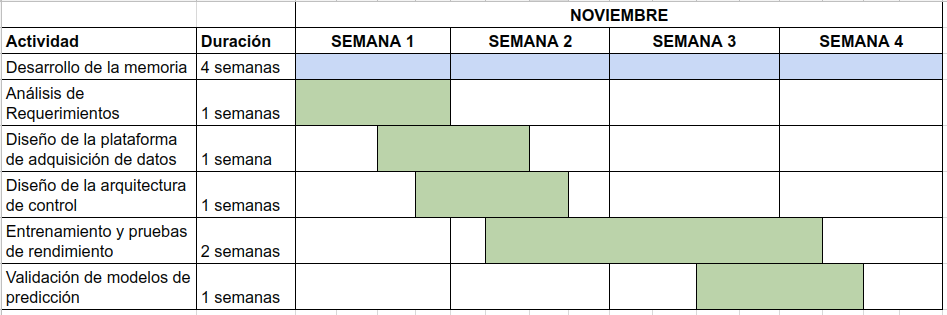
\includegraphics[width=0.85\textwidth]{img/nuevo_cronograma}
    \caption{Diagrama de Gantt para la elaboración del proyecto de grado. Fuente: Elaboración propia}
    \label{fig:cronograma}
    \end{figure}

\newpage
\section{Bibliografia}

\bibliographystyle{IEEEtran}
\bibliography{referencias}
\end{document}
